\section{The availability of neuroimaging data}

\begin{frame}{The size of neuroimaging datasets}
    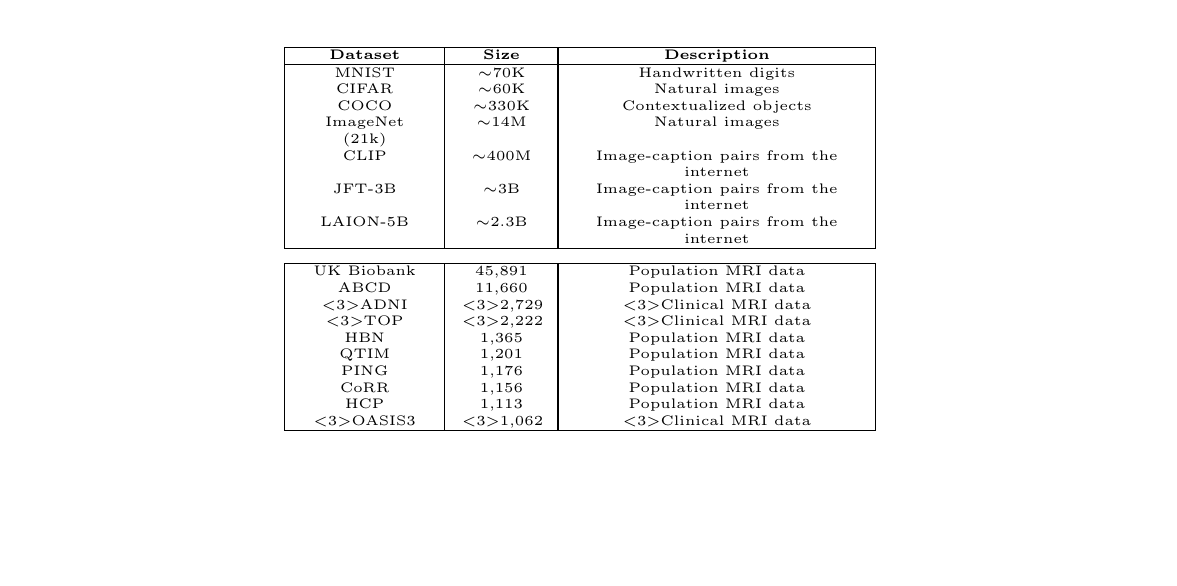
\begin{tikzpicture}
        \node[] at (-7, -3.25) {};
        \node[] at (7, 3.25) {};

        \node[align=center, anchor=north] at (0, 3.25) {
            {\tiny
                \begin{tabular}{|>{\centering\arraybackslash}p{1.6cm}|>{\centering\arraybackslash}p{1cm}|>{\centering\arraybackslash}p{3.6cm}|}
                    \hline
                    \textbf{Dataset}&\textbf{Size}&\textbf{Description}\\
                    \hline
                    MNIST&$\sim$70K&Handwritten digits\\
                    CIFAR&$\sim$60K&Natural images\\
                    COCO&$\sim$330K&Contextualized objects\\
                    ImageNet (21k)&$\sim$14M&Natural images\\
                    CLIP&$\sim$400M&Image-caption pairs from the internet\\
                    JFT-3B&$\sim$3B&Image-caption pairs from the internet\\
                    LAION-5B&$\sim$2.3B&Image-caption pairs from the internet\\
                    \hline
                \end{tabular}
            }
        };

        \only<2-3>{
            \node[align=center, anchor=north] at (0, 0.5) {
                {\tiny
                    \begin{tabular}{|>{\centering\arraybackslash}p{1.6cm}|>{\centering\arraybackslash}p{1cm}|>{\centering\arraybackslash}p{3.6cm}|}
                        \hline
                        UK Biobank&45,891&Population MRI data\\
                        ABCD&11,660&Population MRI data\\
                        \smash{\alert<3>{ADNI}}&\smash{\alert<3>{2,729}}&\smash{\alert<3>{Clinical MRI data}}\\
                        \smash{\alert<3>{TOP}}&\smash{\alert<3>{2,222}}&\smash{\alert<3>{Clinical MRI data}}\\
                        HBN&1,365&Population MRI data\\
                        QTIM&1,201&Population MRI data\\
                        PING&1,176&Population MRI data\\
                        CoRR&1,156&Population MRI data\\
                        HCP&1,113&Population MRI data\\
                        \smash{\alert<3>{OASIS3}}&\smash{\alert<3>{1,062}}&\smash{\alert<3>{Clinical MRI data}}\\
                        \hline
                    \end{tabular}
                }
            };
        }
    \end{tikzpicture}
\end{frame}

\begin{frame}{Transfer learning}
    \begin{tikzpicture}
        \node[] at (-7, -3.25) {};
        \node[] at (7, 3.25) {};

        \only<1-4>{
            \node[draw=black, inner sep=0pt, cm={1,1,0,1,(0,0)}] (input) at (-3.5, 1.3825) {
                \includegraphics[width=0.9cm, height=1.8cm]{data/cat.png}
            };
            \cnnarrow{(input.center)}{($ (input.center) + (2, 0) $)}{black}
            \cnn{-2.7}{1.3825}{0.1}{0.15}{uiogreen}{0}
            \node[anchor=west, align=left, font=\normalfont\linespread{0.9}\selectfont] (output1) at ($ (3.55, 1.3825) + (0, 0.5) $) {Cat};
            \cnnarrow{($ (output1.west) - (1, 0.5) $)}{($ (output1.west) + (0.1, 0) $)}{black}
            \node[anchor=west, align=left, font=\normalfont\linespread{0.9}\selectfont] (output2) at ($ (3.55, 1.3825) - (0, 0.5) $) {Dog};
            \cnnarrow{($ (output2.west) - (1, -0.5) $)}{($ (output2.west) + (0.1, 0) $)}{black}
        }
        \only<2>{
            \node[draw=black, inner sep=0pt] at (-2.5, -1.2) {
                \includegraphics[height=2cm]{
                    data/first.png
                }
            };
            \node[draw=black, inner sep=0pt] at (0, -1.2) {
                \includegraphics[height=2cm]{
                    data/second.png
                }
            };
            \node[draw=black, inner sep=0pt] at (2.5, -1.2) {
                \includegraphics[height=2cm]{
                    data/third.png
                }
            };
        }
        \only<3-4>{
            \node[draw=black, inner sep=0pt, cm={1,1,0,1,(0,0)}] (input) at (-3.5, -1.9) {
                \includegraphics[width=0.9cm, height=1.8cm]{data/caracal.jpg}
            };
            \cnnarrow{(input.center)}{($ (input.center) + (2, 0) $)}{black}
            \cnn{-2.7}{-1.9}{0.1}{0.15}{gray}{0}
            \node[anchor=west, align=left, font=\normalfont\linespread{0.9}\selectfont] (output1) at ($ (3.55, -1.9) + (0, 0.5) $) {Caracal};
            \cnnarrow{($ (output1.west) - (1, 0.5) $)}{($ (output1.west) + (0.1, 0) $)}{black}
            \node[anchor=west, align=left, font=\normalfont\linespread{0.9}\selectfont] (output2) at ($ (3.55, -1.9) - (0, 0.5) $) {Red fox};
            \cnnarrow{($ (output2.west) - (1, -0.5) $)}{($ (output2.west) + (0.1, 0) $)}{black}
        }
        \only<4>{
            \draw[-stealth, uiolightred, line width=0.5, line width=4pt] (-1.75, 0.1) -- (-1.75, -0.6);
            \draw[-stealth, uiolightred, line width=0.5, line width=4pt] (-0.25, 0.35) -- (-0.25, -0.9);
            \draw[-stealth, uiolightred, line width=0.5, line width=4pt] (0.85, 0.78) -- (0.85, -1.3);
            \draw[-stealth, uiolightred, line width=0.5, line width=4pt] (2.1, 1) -- (2.1, -1.5);

        }

    \end{tikzpicture}
\end{frame}

\newcommand{\datasetlegendnode}[2]{
    \node[
        circle,
        anchor=west,
        draw=#1,
        fill=#1!50,
        label={[text depth=0]right:\tiny{#1}},
        inner sep=1.5pt
    ] at (#2){};
}

\newsavebox{\trainingbox}
\sbox{\trainingbox}{
    \definecolor{ds002424}{HTML}{FF0028}
    \definecolor{HBN}{HTML}{FF000E}
    \definecolor{ABCD}{HTML}{FF0C00}
    \definecolor{QTAB}{HTML}{FF2D00}
    \definecolor{PING}{HTML}{FF4800}
    \definecolor{ADHD200}{HTML}{FF6800}
    \definecolor{PNC}{HTML}{FF8300}
    \definecolor{ABIDE-II}{HTML}{FFA400}
    \definecolor{ds000119}{HTML}{FFBF00}
    \definecolor{ABIDE-I}{HTML}{FFDF00}
    \definecolor{BRAINMINT}{HTML}{FFFA00}
    \definecolor{SLIM}{HTML}{E8FF00}
    \definecolor{QTIM}{HTML}{C7FF00}
    \definecolor{Beijing}{HTML}{ACFF00}
    \definecolor{AOMIC-PIOP2}{HTML}{8CFF00}
    \definecolor{ds000202}{HTML}{71FF00}
    \definecolor{AOMIC-PIOP1}{HTML}{51FF00}
    \definecolor{AOMIC-ID1000}{HTML}{36FF00}
    \definecolor{CoRR}{HTML}{15FF00}
    \definecolor{HCP}{HTML}{00FF05}
    \definecolor{FCON1000}{HTML}{00FF20}
    \definecolor{ds000171}{HTML}{00FF40}
    \definecolor{TOP}{HTML}{00FF5B}
    \definecolor{SCZ-C}{HTML}{00FF7B}
    \definecolor{NIMH}{HTML}{00FF96}
    \definecolor{NKI-RS}{HTML}{00FFB6}
    \definecolor{MPI-LEMON}{HTML}{00FFD1}
    \definecolor{ds003592}{HTML}{00FFF1}
    \definecolor{ds004302}{HTML}{00F1FF}
    \definecolor{ds000222}{HTML}{00D5FF}
    \definecolor{SALD}{HTML}{00B5FF}
    \definecolor{IXI}{HTML}{009AFF}
    \definecolor{DLBS}{HTML}{0079FF}
    \definecolor{Cam-CAN}{HTML}{005EFF}
    \definecolor{StrokeMRI}{HTML}{003DFF}
    \definecolor{PPMI}{HTML}{0022FF}
    \definecolor{UKBB}{HTML}{0001FF}
    \definecolor{Tao-Wu}{HTML}{1900FF}
    \definecolor{ds000245}{HTML}{3400FF}
    \definecolor{OASIS3}{HTML}{5500FF}
    \definecolor{Demgen}{HTML}{7000FF}
    \definecolor{NEUROCON}{HTML}{9000FF}
    \definecolor{MIRIAD}{HTML}{AC00FF}
    \definecolor{ds004392}{HTML}{CC00FF}
    \definecolor{AIBL}{HTML}{E700FF}
    \definecolor{ANM}{HTML}{FF00F5}
    \definecolor{ADNI}{HTML}{FF00DA}

    \begin{tikzpicture}
        \begin{axis}[
            width=0.85\textwidth,
            height=0.65\textwidth,
            xmin=0,
            xmax=100,
            ytick=\empty,
            axis x line=middle,
            axis y line=none,
            xtick={10,20,30,40,50,60,70,80,90},
            xticklabels={10,20,30,40,50,60,70,80,{}},
            x axis line style={|-stealth},
            clip=false,
            axis on top,
            tick label style={font=\footnotesize}
        ]
            \pgfplotstableread[col sep=comma]{data/train.csv}\datatable


            \addplot[
                name path=zero,
            ] coordinates {(0,0) (100,0)};

            \pgfplotsinvokeforeach{ABCD, QTAB, PING, PNC, ds000119, SLIM, QTIM, Beijing, AOMIC-PIOP2, ds000202, AOMIC-PIOP1, AOMIC-ID1000, CoRR, HCP, FCON1000, NIMH, NKI-RS, MPI-LEMON, ds003592, ds000222, SALD, IXI, DLBS, Cam-CAN, UKBB, ADNI}{
                \begingroup
                    \addplot [
                        draw=none,
                        line width=0pt,
                        name path=female_#1,
                    ] table [
                        x=age,
                        y expr=1*\thisrow{female_#1}
                    ] {\datatable};

                    \addplot [
                        draw=none,
                        line width=0pt,
                        name path=male_#1,
                    ] table [
                        x=age,
                        y expr=-1*\thisrow{male_#1}
                    ] {\datatable};
                \endgroup
            }
            \pgfplotsinvokeforeach{male, female}{
                \addplot[fill=ABCD!50] fill between[of=zero and #1_ABCD];
                \addplot[fill=QTAB!50] fill between[of=#1_ABCD and #1_QTAB];
                \addplot[fill=PING!50] fill between[of=#1_QTAB and #1_PING];
                \addplot[fill=PNC!50] fill between[of=#1_PING and #1_PNC];
                \addplot[fill=ds000119!50] fill between[of=#1_PNC and #1_ds000119];
                \addplot[fill=SLIM!50] fill between[of=#1_ds000119 and #1_SLIM];
                \addplot[fill=QTIM!50] fill between[of=#1_SLIM and #1_QTIM];
                \addplot[fill=Beijing!50] fill between[of=#1_QTIM and #1_Beijing];
                \addplot[fill=AOMIC-PIOP2!50] fill between[of=#1_Beijing and #1_AOMIC-PIOP2];
                \addplot[fill=ds000202!50] fill between[of=#1_AOMIC-PIOP2 and #1_ds000202];
                \addplot[fill=AOMIC-PIOP1!50] fill between[of=#1_ds000202 and #1_AOMIC-PIOP1];
                \addplot[fill=AOMIC-ID1000!50] fill between[of=#1_AOMIC-PIOP1 and #1_AOMIC-ID1000];
                \addplot[fill=CoRR!50] fill between[of=#1_AOMIC-ID1000 and #1_CoRR];
                \addplot[fill=HCP!50] fill between[of=#1_CoRR and #1_HCP];
                \addplot[fill=FCON1000!50] fill between[of=#1_HCP and #1_FCON1000];
                \addplot[fill=NIMH!50] fill between[of=#1_FCON1000 and #1_NIMH];
                \addplot[fill=NKI-RS!50] fill between[of=#1_NIMH and #1_NKI-RS];
                \addplot[fill=MPI-LEMON!50] fill between[of=#1_NKI-RS and #1_MPI-LEMON];
                \addplot[fill=ds003592!50] fill between[of=#1_MPI-LEMON and #1_ds003592];
                \addplot[fill=ds000222!50] fill between[of=#1_ds003592 and #1_ds000222];
                \addplot[fill=SALD!50] fill between[of=#1_ds000222 and #1_SALD];
                \addplot[fill=IXI!50] fill between[of=#1_SALD and #1_IXI];
                \addplot[fill=DLBS!50] fill between[of=#1_IXI and #1_DLBS];
                \addplot[fill=Cam-CAN!50] fill between[of=#1_DLBS and #1_Cam-CAN];
                \addplot[fill=UKBB!50] fill between[of=#1_Cam-CAN and #1_UKBB];
                \addplot[fill=ADNI!50] fill between[of=#1_UKBB and #1_ADNI];
            }

            \node[
                anchor=south east,
                font=\footnotesize
            ] at (axis cs: 99, 0.0){FEMALE};
            \node[
                anchor=north east,
                font=\footnotesize
            ] at (axis cs: 99, -0.0){MALE};

            \def\xdiff{35.5}
            \def\xmin{102}
            \def\ydiff{0.07}
            \def\ymin{12.5*\ydiff}

            \datasetlegendnode{ABCD}{axis cs: \xmin, \ymin}
            \datasetlegendnode{QTAB}{axis cs: \xmin, \ymin-\ydiff}
            \datasetlegendnode{PING}{axis cs: \xmin, \ymin-2*\ydiff}
            \datasetlegendnode{PNC}{axis cs: \xmin, \ymin-3*\ydiff}
            \datasetlegendnode{ds000119}{axis cs: \xmin, \ymin-4*\ydiff}
            \datasetlegendnode{SLIM}{axis cs: \xmin, \ymin-5*\ydiff}
            \datasetlegendnode{QTIM}{axis cs: \xmin, \ymin-6*\ydiff}
            \datasetlegendnode{Beijing}{axis cs: \xmin, \ymin-7*\ydiff}
            \datasetlegendnode{AOMIC-PIOP2}{axis cs: \xmin, \ymin-8*\ydiff}
            \datasetlegendnode{ds000202}{axis cs: \xmin, \ymin-9*\ydiff}
            \datasetlegendnode{AOMIC-PIOP1}{axis cs: \xmin, \ymin-10*\ydiff}
            \datasetlegendnode{AOMIC-ID1000}{axis cs: \xmin, \ymin-11*\ydiff}
            \datasetlegendnode{CoRR}{axis cs: \xmin, \ymin-12*\ydiff}
            \datasetlegendnode{HCP}{axis cs: \xmin, \ymin-13*\ydiff}
            \datasetlegendnode{FCON1000}{axis cs: \xmin, \ymin-14*\ydiff}
            \datasetlegendnode{NIMH}{axis cs: \xmin, \ymin-15*\ydiff}
            \datasetlegendnode{NKI-RS}{axis cs: \xmin, \ymin-16*\ydiff}
            \datasetlegendnode{MPI-LEMON}{axis cs: \xmin, \ymin-17*\ydiff}
            \datasetlegendnode{ds003592}{axis cs: \xmin, \ymin-18*\ydiff}
            \datasetlegendnode{ds000222}{axis cs: \xmin, \ymin-19*\ydiff}
            \datasetlegendnode{SALD}{axis cs: \xmin, \ymin-20*\ydiff}
            \datasetlegendnode{IXI}{axis cs: \xmin, \ymin-21*\ydiff}
            \datasetlegendnode{DLBS}{axis cs: \xmin, \ymin-22*\ydiff}
            \datasetlegendnode{Cam-CAN}{axis cs: \xmin, \ymin-23*\ydiff}
            \datasetlegendnode{UKBB}{axis cs: \xmin, \ymin-24*\ydiff}
            \datasetlegendnode{ADNI}{axis cs: \xmin, \ymin-25*\ydiff}

            \node[align=center, font=\small\linespread{0.9}\selectfont] at (axis cs: 50, -0.6) {
                68,570 MRIs\\59,923 participants\\26 sources
            };
        \end{axis}
    \end{tikzpicture}
}

\newcommand{\resultstrace}[3]{
    \addplot+[
        scatter,
        draw=#2,
        mark=#3,
        thick,
        draw opacity=0.75,
        visualization depends on={\thisrow{#2-significant} \as \significant},
        scatter/@pre marker code/.code={
            \pgfplotscolormapdefinemappedcolor\pgfplotspointmetatransformed
            \def\markopts{
                fill=#2,
                fill opacity=0.75*\significant,
                mark size=4pt
            }
            \expandafter\scope\expandafter[\markopts]
        },
    ] table [
        col sep=comma,
        x=size,
        y=#2-median,
        meta=#2-significant
    ] {#1};
}
\newcommand{\legendtrace}[3][0.75]{
    \begin{tikzpicture}[baseline={([yshift=-0.125cm]current bounding box.center)}]
        \draw[draw=#2, thick] (0cm, 0cm) -- (0.5cm, 0cm);

        \path[
            mark=#3,
            mark size=4pt,
            mark options={fill=#2, draw=#2},
            fill opacity=#1
        ] plot coordinates {(0.25cm, 0cm)};
    \end{tikzpicture}
}

\newcommand{\legendnode}[4][north east]{
    \node[draw=black, fill=white, anchor=#1, font=\fontsize{6}{5}\selectfont, text width=3.3cm] at (#2) {
        \vspace{-0.07cm}
        \setlength\tabcolsep{0cm}
        \renewcommand{\arraystretch}{1.8}
        \begin{tabular}{p{0.53cm} p{2.8cm}}
            #3
        \end{tabular}
        \vspace{0.2cm}\\
        \begin{tabular}{p{0.53cm} p{2.8cm}}
            #4
        \end{tabular}
    };
}

\definecolor{multi-transferred}{RGB}{213, 94, 0}
\definecolor{multi-frozen}{RGB}{0, 158, 115}
\definecolor{multi-finetuned}{RGB}{86, 180, 233}
\definecolor{reg-finetuned}{RGB}{213, 94, 0}
\definecolor{baseline}{RGB}{230, 159, 0}
\definecolor{linear}{RGB}{64, 64, 64}

\makeatletter
\pgfdeclareplotmark{triangledown*}{
  \pgfpathmoveto{\pgfpoint{0}{-1.2\pgfplotmarksize}}
  \pgfpathlineto{\pgfpoint{1.04\pgfplotmarksize}{0.6\pgfplotmarksize}}
  \pgfpathlineto{\pgfpoint{-1.04\pgfplotmarksize}{0.6\pgfplotmarksize}}
  \pgfpathclose
  \pgfusepathqfillstroke
}
\makeatother

\def\multifrozenmarker{*}
\def\regfinetunedmarker{square*}
\def\multifinetunedmarker{pentagon*}
\def\multitransferredmarker{triangle*}
\def\linearmarker{triangledown*}
\def\baselinemarker{diamond*}


\newcommand{\adhc}{
    \begin{tikzpicture}
        \begin{axis}[
            height=7cm,
            width=12cm,
            ymajorgrids=true,
            xlabel={Training dataset size},
            ylabel={Area under the ROC-curve},
            tick style={draw=none},
            xtick={100, 200, 300, 400, 500},
            xlabel style={
                yshift=0.1cm
            },
            ymin=0.65,
            ymax=0.97
        ]
            \resultstrace{data/downstream/ad/results.csv}{baseline}{\baselinemarker}

            \node[draw=black, fill=white, anchor=south east, text width=3.4cm, inner sep=2pt, font=\footnotesize] at (rel axis cs: 0.98, 0.02) {
                \setlength\tabcolsep{0cm}%
                \begin{tabular}{cl}
                    \legendtrace{baseline}{\baselinemarker} & Baseline model\\
                    \visible<4->{\legendtrace{multi-finetuned}{\multifinetunedmarker}} & \visible<4->{Transfer learning}\\
                \end{tabular}

            };

            \only<4->{
                \resultstrace{data/downstream/ad/results.csv}{multi-finetuned}{\multifinetunedmarker}
            }

        \end{axis}
    \end{tikzpicture}
}

\begin{frame}{Transfer learning on neuroimaging data}
    \begin{tikzpicture}
        \node[draw=black] at (-7, -3.25) {};
        \node[draw=black] at (7, 3.25) {};

        \only<1>{
            \node[] at (0, 0) {
                \hspace{-4.5cm}\usebox{\trainingbox}
            };
        }
        \only<2>{
            \inputside{-4.5}{0}{1.5cm}
            \cnnarrow{(input.east)}{($ (input.center) + (2.5, 0) $)}{black}
            \cnn{-2.7}{0}{0.1}{0.15}{uiogreen}{0}
            \node[anchor=west, align=left, font=\normalfont\linespread{0.9}\selectfont] (output1) at (3.55, 0) {Brain age};
            \cnnarrow{($ (output1.west) - (1, 0) $)}{($ (output1.west) + (0.1, 0) $)}{black}
            \node[anchor=west, align=left, font=\normalfont] (output1) at (3.55, 1.66) {Brain age};
            \cnnarrow{($ (output1.west) - (1, 1.66) $)}{($ (output1.west) + (0.1, 0) $)}{black}
            \node[anchor=west, align=left, font=\normalfont] (output2) at (3.55, 1) {Sex};
            \cnnarrow{($ (output2.west) - (1, 1) $)}{($ (output2.west) + (0.1, 0) $)}{black}
            \node[anchor=west, align=left, font=\normalfont] (output3) at (3.55, 0.33) {Handedness};
            \cnnarrow{($ (output3.west) - (1, 0.33) $)}{($ (output3.west) + (0.1, 0) $)}{black}
            \node[anchor=west, align=left, font=\normalfont] (output4) at (3.55, -0.33) {BMI};
            \cnnarrow{($ (output4.west) - (1, -0.33) $)}{($ (output4.west) + (0.1, 0) $)}{black}
            \node[anchor=west, align=left, font=\normalfont\linespread{0.8}\selectfont] (output5) at (3.55, -1) {Fluid\\intelligence};
            \cnnarrow{($ (output5.west) - (1, -1) $)}{($ (output5.west) + (0.1, 0) $)}{black}
            \node[anchor=west, align=left, font=\normalfont] (output6) at (3.55, -1.66) {Neuroticism};
            \cnnarrow{($ (output6.west) - (1, -1.66) $)}{($ (output6.west) + (0.1, 0) $)}{black}

        }
        \only<3-4>{
            \node[] at (0, 0) {
                \adhc
            };
        }
    \end{tikzpicture}
\end{frame}

\begin{frame}{Transfer learning on neuroimaging data}
    Training modern artificial neural networks require \textit{really} large datasets (millions or billions of training examples).
    \begin{itemize}
        \item Existing neuroimaging datasets are relatively small (tens of thousands of participants), a problem further exacerbated in clinical datasets (thousands of participants).
        \item Transfer learning represents a promising approach for training complex models with limited data.
    \end{itemize}
\end{frame}